\documentclass[a4paper]{article}
\usepackage{amsfonts}
\usepackage{amsmath}
\usepackage{amssymb}
\usepackage{graphicx}
\begin{document}

\noindent \large Auteur: Anass Hamzaoui \\
\noindent \large Studierichting: Informatica \\
\noindent \large Oefeningenreeks 5F nr. 4 \\
\medskip
\normalsize

$9y^2 = x(x-3)^2$ \\

$\left|\begin{array}{ll}
    & \text{Symmetrie: } y^2 \implies \text{symmetrisch t.o.v. de } x\text{-as} \\
    
    & \text{Domein: } x(x-3)^2 \geq 0 \implies x \geq 0 \\
    
    & \text{Snijpunten met } x\text{-as: } y = 0 \implies x(x-3)^2 = 0 \implies x = 0 \text{ en } x = 3 \\
    
    & \text{Bovenste helft: } y = \dfrac{1}{3}(3-x)\sqrt{x} = \sqrt{x} - \dfrac{1}{3}x^{3/2} \\
    
    & \text{Maximum: } y' = 0 \implies x = 1 \implies \left(1, \dfrac{2}{3}\right), \text{ minimum: } \left(1, -\dfrac{2}{3}\right) \\
\end{array}\right.$ \\

Grafiek: \\
\begin{figure}[h]
\centering
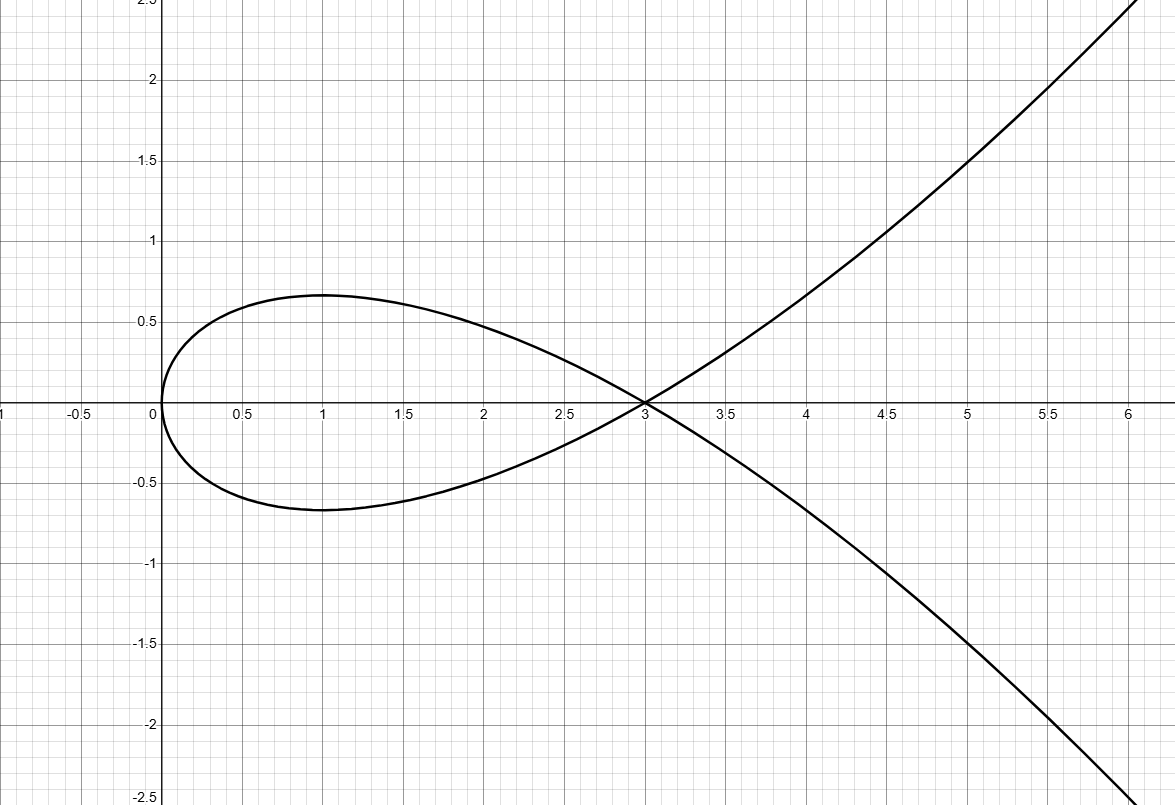
\includegraphics[width=8cm]{5I-4-anass.hamzaoui.INF.png}
\end{figure}

$\begin{array}{ll}
L &= 2\displaystyle\int_0^3 \sqrt{1+(y')^2} \, dx \\

y &= x^{1/2} - \dfrac{1}{3}x^{3/2} \implies y' = \dfrac{1}{2}x^{-1/2} - \dfrac{1}{2}x^{1/2} = \dfrac{1-x}{2\sqrt{x}} \\

(y')^2 &= \dfrac{(1-x)^2}{4x} = \dfrac{1-2x+x^2}{4x} \\

1+(y')^2 &= \dfrac{4x+1-2x+x^2}{4x} = \dfrac{(x+1)^2}{4x} \\

\sqrt{1+(y')^2} &= \dfrac{x+1}{2\sqrt{x}} = \dfrac{1}{2}x^{-1/2} + \dfrac{1}{2}x^{1/2} \\

L &= 2\displaystyle\int_0^3 \left(\dfrac{1}{2}x^{-1/2} + \dfrac{1}{2}x^{1/2}\right) dx \\

&= 2\left[x^{1/2} + \dfrac{1}{3}x^{3/2}\right]_0^3 \\

&= 2\left(\sqrt{3} + \dfrac{1}{3}\cdot 3\sqrt{3}\right) \\

&= 2 \cdot 2\sqrt{3} = 4\sqrt{3} \\
\end{array}$

\begin{thebibliography}{999}
    %\bibitem{a} Referentie
\end{thebibliography}
\end{document}